%%%%%%%%%%%%%%%%%%%%%%%%%%%%%%%%%%%%%%%%%%%%%%%%%%%%%%%%%%%%%%%%%%% 
%                                                                 %
%                          Spatial Analysis                       %
%                                                                 %
%%%%%%%%%%%%%%%%%%%%%%%%%%%%%%%%%%%%%%%%%%%%%%%%%%%%%%%%%%%%%%%%%%% 

\chapter{Análisis Estadístico Espacial}
%\resetfootnote %this command starts footnote numbering with 1 again.
Este capítulo pretende introducir algunos métodos para analizar datos espaciales cuantitativos. \textit{Espacial} significa que cada elemento de los datos tiene referencia geográfica de tal manera que podamos saber en qué parte del mapa ocurre cada caso. Dicha referencia espacial es importante porque acarrea información relevante para el análisis de los datos.

\section{¿Qué es el análisis espacial?}
El término ``análisis espacial'' es muy utilizado en la literatura de  los Sistemas de Información Geográfica (GIS por sus siglas en inglés)  y de Ciencia de Información Geográfica (GISc por sus siglas en inglés). El análisis espacial es un conjunto de técnicas y modelos que usan la referencia espacial asociada a cada individuo de los datos. Los métodos de análisis espacial necesitan hacer supuestos para describir la asociación o interacción espacial entre los casos. Los resultados de cualquier análisis espacial no son los mismos bajo re-arreglos de la distribución espacial o reconfiguraciones de la estructura espacial del sistema bajo investigación.

El análisis espacial tiene tres elementos principales:

\begin{enumerate}
\item \textit{Modelado cartográfico}. El conjunto de datos es representado como un mapa y las operaciones basadas en mapas generan nuevos mapas.

\item \textit{Modelado matemático}. Las salidas del modelo dependen de la forma de modelar la interacción espacial entre los objetos, de las relaciones espaciales o del posicionamiento geográfico de los objetos dentro del modelo.

\item \textit{Análisis estadístico espacial}. Consiste en el desarrollo y la aplicación de técnicas estadísticas para analizar los datos espaciales, por consiguiente, hace uso de las referencias espaciales en el conjunto de datos.

Se debe de tener cuidado al hacer el análisis estadístico. A pesar de que el análisis de dependencia espacial es una pieza clave del análisis estadístico espacial, si se pone demasiada atención a las características espaciales de los datos, se pueden llegar a ignorar otras características importantes de estos. El análisis estadístico espacial es sólo un subcampo del análisis estadístico. Para hacer un análisis correcto de los datos espaciales, hay un rol muy importante de las otras áreas de la teoría estadística donde no se involucra el uso de datos espaciales.

\end{enumerate}

\section{Estadística Espacial}
Los datos espaciales se distinguen por observaciones obtenidas en ubicaciones espaciales $s_1,s_2,\dots,s_n$ donde $s_i$ pueden ser coordenadas en el plano $\Re^2$ ó $\Re^3$ , líneas que unen un punto con otro o polígonos que cubren un área determinada (e.g. países, regiones o lagos).

Los modelos espaciales intentan modelar la correlación entre observaciones en diferentes posiciones en el espacio.
En estadística espacial, se cuenta principalmente con tres tipos de análisis de datos:

\begin{itemize}

\item \textbf{Geoestadística}. Se caracteriza por datos que involucran la medición de la variable de interés sobre una región espacial (e.g. país, municipio, lago) donde la medición de los datos puede variar de manera continua.

Sea $D$ la región de interés, cada punto $s=(x,y)$ en $D$ puede ser descrito por un par coordenado $x$ y $y$ en el plano.

\item \textbf{Patrón de Puntos Espaciales}. Consideremos la región $D$, en ésta estamos interesados en la ubicación de ciertos ``eventos''. Nos preguntamos si los eventos de interés ocurren de manera aleatoria a lo largo del área o si los eventos tienden a aglomerarse.

El problema con tratar de determinar la presencia de aglomeraciones en un conjunto de datos espaciales, puede ser muy complicado. Puntos generados de manera completamente aleatoria, pueden parecer aglomerados

\item \textbf{Datos en retícula}. Determinamos la región $D$ como una colección finita de sitios espaciales donde se llevan a cabo las observaciones. A la colección de puntos en $D$ se le conoce como celosía o retícula (en inglés, ``lattice'').  Dichos sitios espaciales en la retícula, son identificados normalmente utilizando su longitud y latitud.

Hay tres características de los datos en celosía a tomar en cuenta:
\begin{enumerate}
\item ¿La retícula es regular o irregular? Por ejemplo, los estados de México son irregulares; pero, por otro lado, podemos tener mediciones sobre un campo agrícola particionado en bloques regulares.
\item ¿Las ubicaciones en la celosía hacen referencia a ``puntos'' o ``regiones''? En los estados de México, cada estado es una región.
\item ¿La variable de interés es categórica o numérica?

Una forma sencilla de ilustrar gráficamente los datos en retícula es utilizando un \textit{mapa coroplético}. Un mapa coroplético es un mapa que muestra las regiones o áreas con características similares. Por ejemplo, si queremos ver el índice de marginación en México dividido por municipio, como se ve en la Figura \ref{map_marg_ej} los municipios con índices similares tienen colores similares.

\begin{figure}[!ht]
\centering
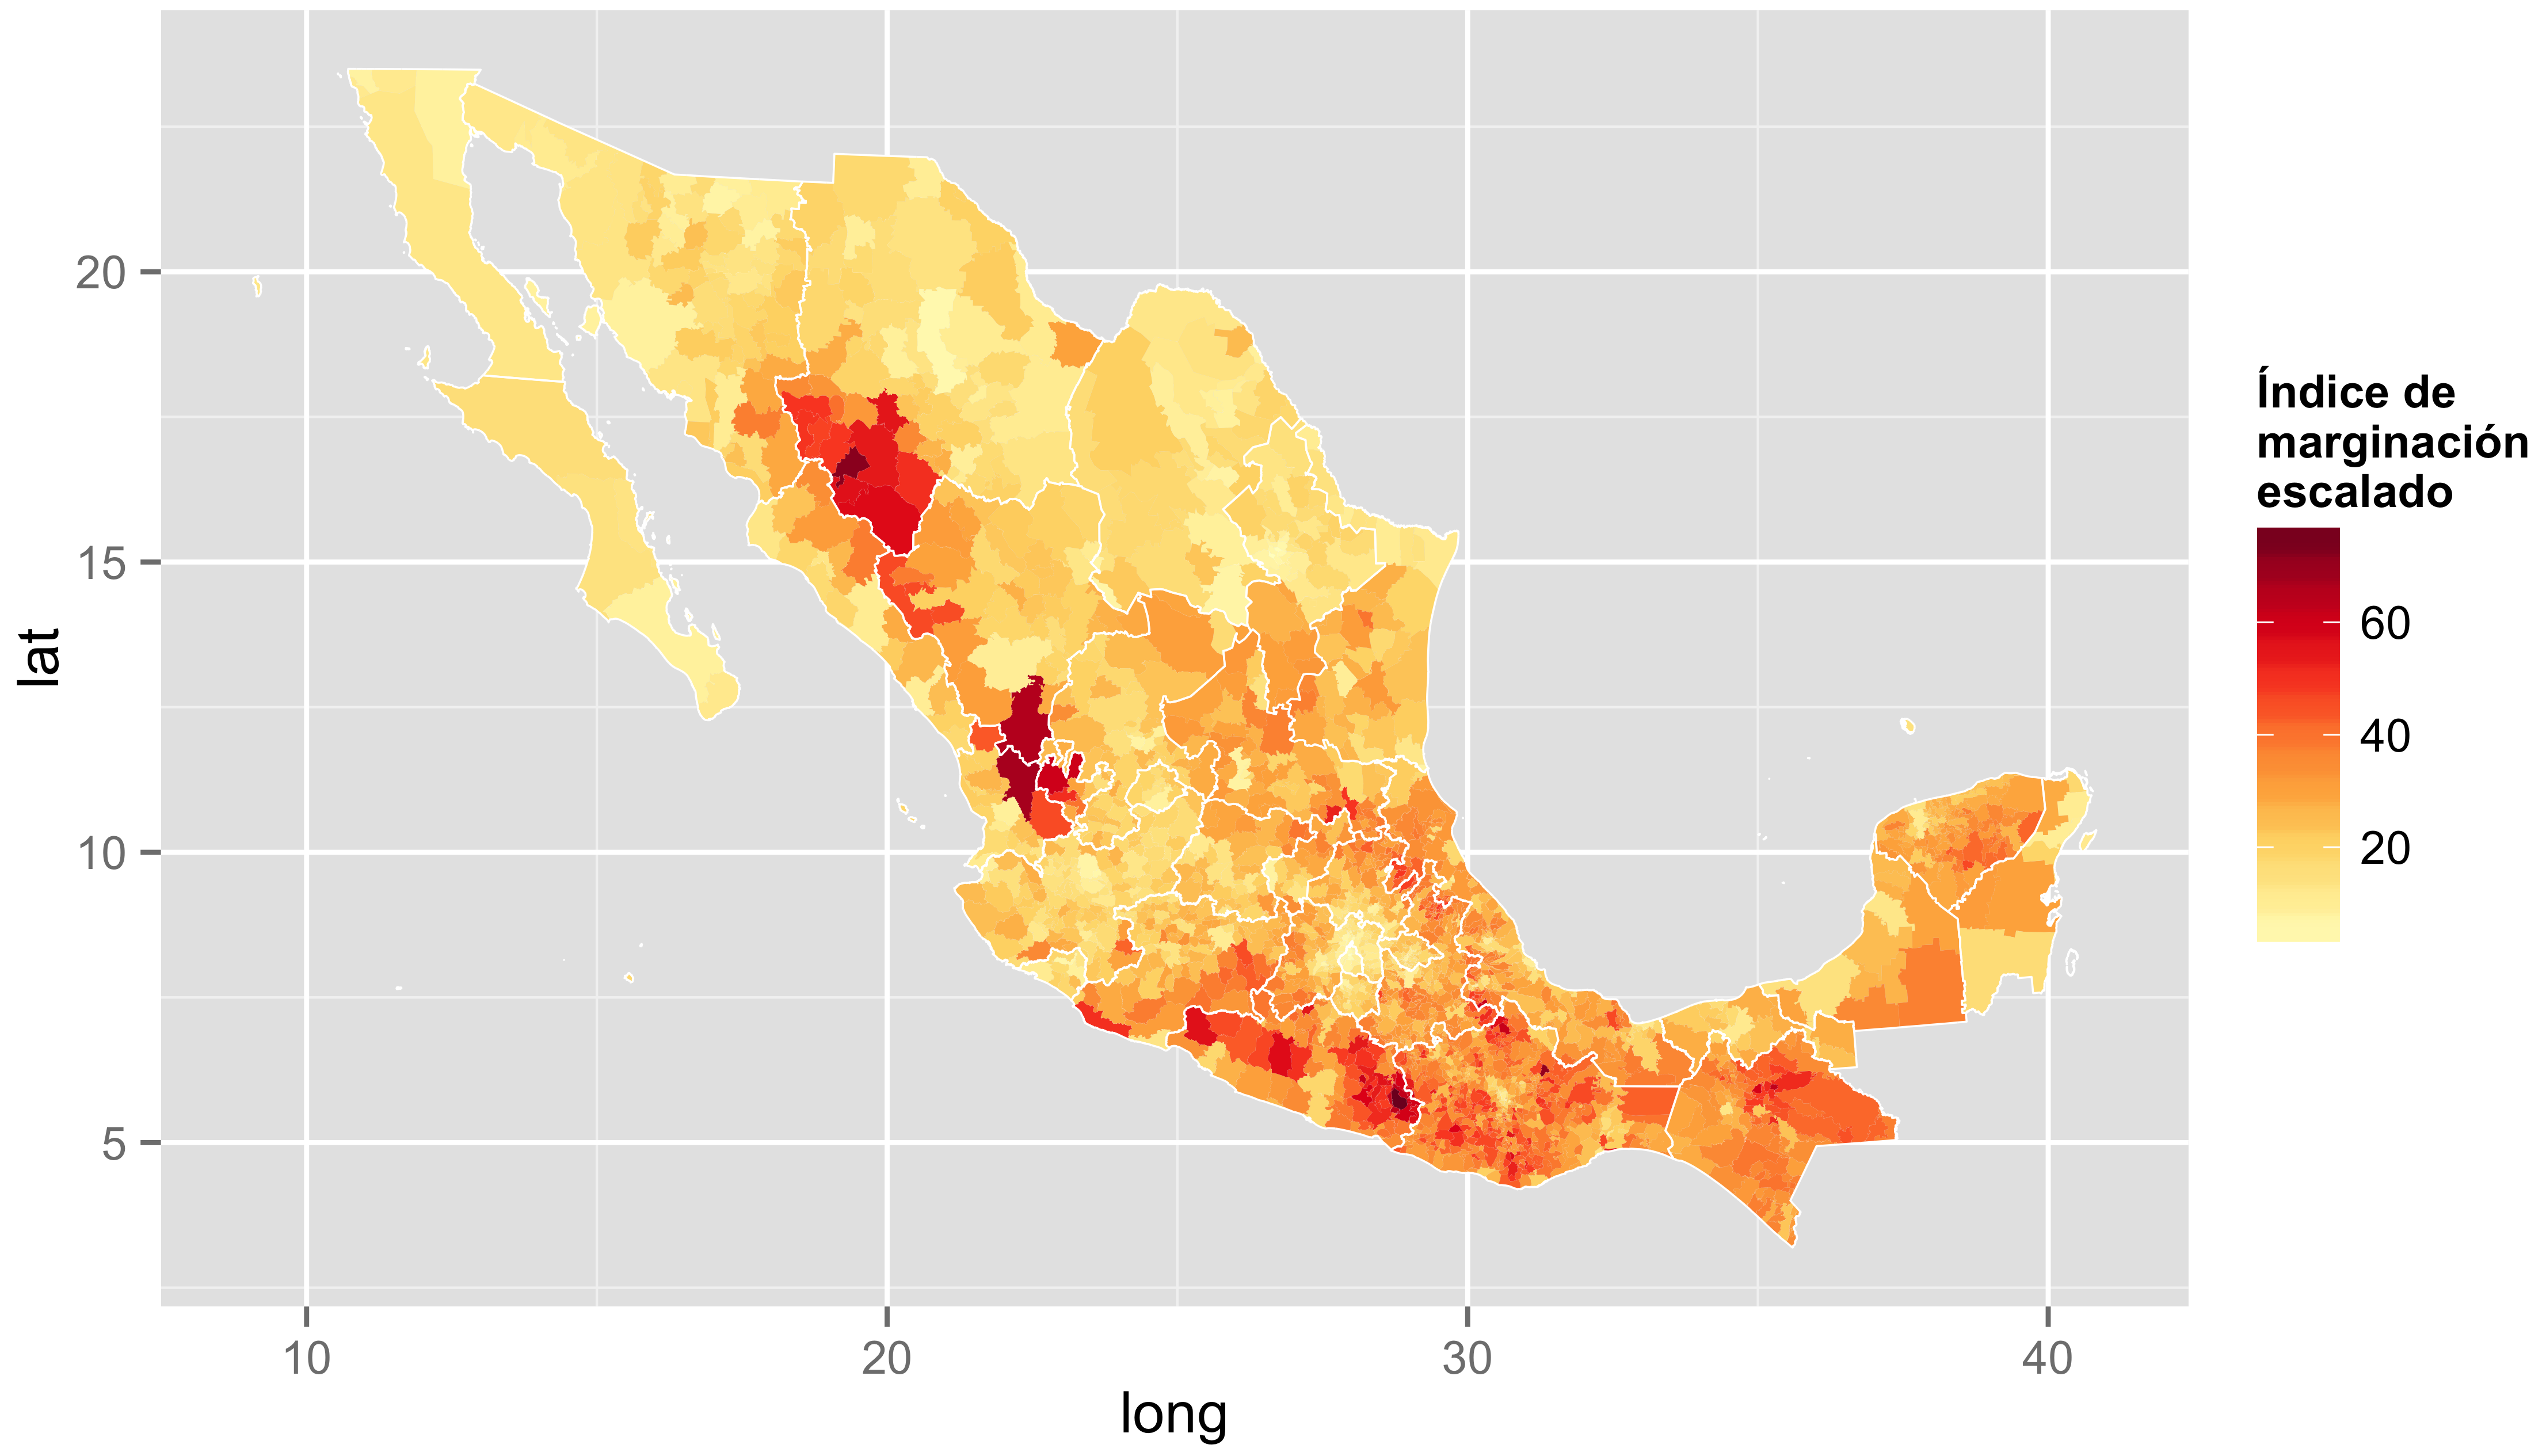
\includegraphics[width=.9\textwidth]{./maps/mapmarg.png} \\
\caption{ Índice de marginación por municipio.}
\label{map_marg_ej}  
\end{figure}

\end{enumerate}

\end{itemize}


\chapter{Autocorrelación Espacial}

Las observaciones realizadas en diferentes puntos espaciales pueden no ser independientes. Por ejemplo,  medidas obtenidas en lugares cercanos pueden ser más parecidas que en lugares lejanos. A esto se le llama autocorrelación espacial, la cual mide el grado en el que un fenómeno de interés se relaciona consigo mismo en el espacio \citep{clifford1973, clifford1981}.

Las pruebas de autocorrelación espacial examinan si el valor observado de una variable en algún lugar  es independiente de valores de la misma variable en lugares cercanos o  contiguos.

Un índice de \textit{autocorrelación espacial global} resume el nivel de similitud espacial observada entre las observaciones vecinas sobre el área entera estudiada.

\begin{itemize}
\item \textbf{Autocorrelación espacial positiva} indica que los valores similares están cercanos entre sí, o aglomerados, en el espacio.
\item \textbf{Autocorrelación espacial negativa} indica que valores vecinos no son similares, o equivalentemente, que valores similares están dispersos en el espacio.
\item \textbf{Autocorrelación espacial nula} indica que el patrón espacial es aleatorio.
\end{itemize}

La mayoría de los índices de autocorrelación comparten una estructura común. En dicha estructura, se calcula la similitud entre valores en las localidades $i$ y $j$, luego se pondera dicha similitud por la proximidad entre éstos. Altas similitudes con mucho peso provocan un valor alto del índice, mientras que bajas similitudes con mucho peso provocan un valor bajo del índice.

\section{Matriz de Pesos}
Para evaluar la autocorrelación espacial, se debe definir primero qué significa que dos observaciones sean cercanas, es decir, se debe definir una métrica de distancia. Dichas distancias son presentadas en una matriz de pesos en la cual se define la relación entre los diferentes lugares donde se obtuvieron las observaciones. Si los datos fueron obtenidos en $n$ lugares distintos, entonces la matriz de pesos $W$ es de $n \times n$, donde cada entrada $w_{ij}$, $i,j=1, 2, \dots, n$ representa la dependencia espacial o peso entre los lugares $i$ y $j$ definiendo así la estructura de los vecinos sobre el área entera. \citet{haining} presenta las siguientes maneras para construir los pesos:

\begin{itemize}
\item  \textbf{Contigüidad binaria}: Es la definición de pesos más sencilla, se define como 

\begin{equation} \label{binw}
w_{ij}=  \begin{cases} 1 & \mbox{si la región } i \mbox{ comparte frontera con } j \\ 
0 & \mbox{e.o.c.} 
\end{cases}
\end{equation}.

Nótese que con dicha elección de medida de proximidad $W$ es necesariamente simétrica , pues $w_{ij}=w_{ji}$.


\item \textbf{Distancia}: Se definen los pesos como $w_{ij}=d_{ij}^{-\delta}$ donde $d_{ij}$ denota la distancia entre $i$ y $j$ y el parámetro $\delta \geq 0$. La distancia puede definirse de distintas maneras (e.g. distancia Euclideana).

\item \textbf{Función exponencial de distancia}: Se define como $w_{ij}=e^{d_{ij}^{-\delta}}$.

\item \textbf{Frontera en común}: Sean $l_{ij}$ la longitud de la frontera entre $i$ y $j$ y $l_i$ la longitud de la frontera de la región $i$, se pueden definir los pesos como $w_{ij}=\left( \dfrac{l_{ij}}{l_i}\right)^{\tau}$ con $\tau \geq 0$.

\item \textbf{Combinación de frontera y distancia}: Es una combinación entre los pesos por distancia y por tamaño de frontera, se define como $w_{ij}=\left( \dfrac{l_{ij}}{l_i}\right)^{\tau}d_{ij}^{-\delta}$ donde $\tau, \delta \geq 0$.
\end{itemize}

\textbf{Nota}: Para todos los casos  $w_{ii}=0$ y $w_{ij} \geq 0$ para $i,j=1,2,...,n$, obteniendo así una matriz de la siguiente forma,

\begin{equation}
W= \begin{pmatrix}
 0 & w_{12} & \cdots & w_{1n} \\
 w_{21} & 0 & \cdots & w_{2n}  \\
 \vdots & \vdots & \ddots & \vdots \\
 % w_{n-1,1} & \vdots & \ddots & w_{n-1,n}\\
 w_{n1} & w_{n2} & \cdots & 0  \\
\end{pmatrix}.
\end{equation}

Podemos ajustar $W$ de tal forma que la suma de los pesos por renglón sea igual a $1$  utilizando una matriz estandarizada por filas donde dividimos cada elemento $w_{ij}$ por la suma de los pesos de los vecinos de la región $i$ obteniendo una matriz $W_{std}$ donde

\begin{equation}
w_{std,ij}=\dfrac{w_{ij}}{\displaystyle \sum_{j=1}^n w_{ij}}.
\end{equation}

En el caso de los pesos binarios, dicha estandarización penaliza los pesos de las regiones con muchos vecinos.


\section{Pruebas de Autocorrelación Espacial Global}
Consideremos un área de estudio particionada en $n$ regiones. Sea $Y$ la variable de estudio, $y_i$ es la observación de la variable $Y$ en la región $i$.  Para cada par de regiones $i$ y $j$, si las observaciones $y_i$ y $y_j$ no están correlacionadas, entonces decimos que no hay autocorrelación espacial en el área de estudio para la variable $Y$. De manera inversa, decimos que existe autocorrelación espacial si las observaciones están correlacionadas por pares. Las pruebas de autocorrelación espacial propuestas en la literatura, dependen del tipo de la variable de estudio (discreta, ordinal o continua).

\subsection{Variables continuas u ordinales}
Si $Y$ es de escala continua u ordinal, utilizamos dos coeficientes que miden el grado de autocorrelación entre las $y_i$'s en regiones unidas, donde $y_i$ es una observación en la región $i$.
% % Si $X$ se distribuye $N(\mu, \sigma^2)$

% \subsubsection{Prueba }
% Supongamos que se cuenta $n$ regiones (e.g. municipio o estados) y que contamos con medidas de una variable $y$ para cada región.
%  \# Falta hablar sobre los supuestos y las pruebas de hipótesis \#



\subsubsection{Índice $\mathcal{I}$ de Moran} 
El índice $\mathcal{I}$ de Moran propuesto por \citet{moran50} sirve para probar la autocorrelación espacial global para variables continuas. Se basa en los productos cruzados de las desviaciones de la media y se calcula para  $n$ observaciones de una variable $y$ en lugares $i,j$ como sigue:

\begin{equation}
\mathcal{I} = \left( \dfrac{n}{\displaystyle \sum_{i=1}^n \sum_{j=1}^n w_{ij}} \right) \left( \dfrac{\displaystyle \sum_{i=1}^n \sum_{j=1}^n w_{ij} (y_{i} - \bar{y}) (y_{j} - \bar{y}) }{\displaystyle \sum_{i=1}^n (y_{i} - \bar{y})^2} \right).
\end{equation}

$y_{i}$ es el valor de la variable en el lugar $i$ y $\overline{y}$ es la media muestral.

$\mathcal{I}$ no es como un coeficiente de correlación común, pues no pertenece necesariamente al intervalo $(-1,1)$. Usualmente $\mathcal{I} \in (-1,1)$, a menos que se cuente con regiones con valores extremos de $y_{i} - \overline{y}$ con pesos muy altos.


\subsubsection{Índice $\mathcal{C}$ de Geary} 
El índice $\mathcal{C}$ de Geary utiliza la suma de diferencias al cuadrado entre pares de observaciones como medida de variación. Fue sugerido por \citet{geary54} y está dado por

\begin{equation}
\mathcal{C} =  \left(\dfrac{n-1}{\displaystyle 2 \sum_{i=1}^n \sum_{j=1}^n w_{ij}}\right)  \left( \dfrac{\displaystyle \sum_{i=1}^n \sum_{j=1}^n w_{ij} (y_{i} - y_{j})^2}{\displaystyle \sum_{i=1}^n (y_{i} - \hat{y})^2}\right).
\end{equation}

El índice $\mathcal{C}$ de Geary toma valores en el intervalo $[0,2]$ donde 0 indica correlación espacial positiva perfecta (i.e. $y_{i}=y_{j}$ para cualquier par de regiones donde $w_{ij}>0$ y 2 indica correlación espacial negativa perfecta. 

$\mathcal{C}$ no es propiamente un coeficiente de correlación, en cambio, corresponde a una estadístico $d$ de Durbin-Watson \citep{clifford1981}, utilizada para probar autocorrelación serial en análisis de regresión y en análisis de series de tiempo.

En contraste con $\mathcal{I}$ , valores bajos de $\mathcal{C}$ denotan autocorrelación espacial positiva y valores altos indican autocorrelación espacial negativa.


Ambos índices $\mathcal{I}$ y $\mathcal{C}$ tienen la forma clásica de un coeficiente de autocorrelación: el numerador en cada uno es una medida de covarianza entre las $y_i$'s y el denominador es una medida de varianza. Es evidente también que $\mathcal{I}$  está basado en productos cruzados de las desviaciones entre $y_i$ y $\bar{y}$ , opuesto a las diferencias cuadráticas entre las $y_i$'s del coeficiente de Geary.

Se puede mostrar \citep[Capítulo 2]{clifford1973} que  $\mathcal{I}$ y $\mathcal{C}$ asíntóticamente, se distribuyen normal a medida que $n$ aumenta. Los momentos de $\mathcal{I}$ y $\mathcal{C}$ pueden ser evaluados bajo alguna de los siguientes dos supuestos:

\begin{enumerate}
\item \textbf{Normalidad}. Bajo este supuesto, asumimos que las observaciones $y_i$ son resultado de $n$ realizaciones de una población normal.
\item \textbf{Aleatorización}. Independientemente de la distribución subyacente de la población, consideramos el valor observado de $\mathcal{I}$ y $\mathcal{C}$ relativo al conjunto de todos los valores posibles que pueden tomar $\mathcal{I}$ y $\mathcal{C}$ si $y_1, y_2, ..., y_n$ fueran permutadas de manera aleatoria repetidamente alrededor de las regiones dentro del área de estudio. Hay $n!$ valores posibles.
\end{enumerate}

Usando los subíndices N y R para denotar los supuestos de normalidad y aleatorización respectivamente. Si utilizamos pesos $w_{ij}$ simétricos (i.e. $w_{ij}=w_{ji}$) se puede probar que los momentos de los índices quedan como sigue.

\subsubsection*{Coeficiente $\mathcal{I}$}
\begin{align}
\EN\left[\mathcal{I} \right]  = &\ER \left[\mathcal{I}\right]=-\dfrac{1}{n-1},\\
\EN\left[\mathcal{I}^2\right] = & \dfrac{n^2S_1-nS_2+3S_0^2}{S_0^2(n^2-1)}, \\
\ER\left[\mathcal{I}^2\right] = &\dfrac{n \left[ (n^2-3n+3)S_1 - nS_2 + 3S_0^2 \right] - b_2 \left[ (n^2 - n)S_1 - 2nS_2 +6S_0^2\right]}{(n-1)(n-2)(n-3)S_0^2}.
\end{align}

\subsubsection*{Coeficiente $\mathcal{C}$}
\begin{align}
\EN\left[\mathcal{C}\right] = &\left[\mathcal{C}\right] = 1, \\
\VarN(\mathcal{C}) =&\dfrac{(2S_1+S_2)(n-1)-4S_0^2}{2(n+1)S_0^2}, \\
\VarR(\mathcal{C}) =& \Big( (n-1)S_1 \left[ n^2 -3n +3 -(n-1)b_2 \right] \\ \nonumber
   &- \frac{1}{4} (n-1)S_2 \left[ n^2 +3n -6 -(n^2-n+2)b_2 \right] \\ \nonumber
  &+ S_0^2 \left[ n^2 -3 - (n-1)^2 b_2 \right] \Big) \left( \dfrac{1}{n(n-2)(n-1)S_0^2} \right). \nonumber
\end{align}

Donde 
\begin{align}
  S_0 =& \sum_{i=1}^n \sum_{j=1}^n w_{ij}, \\
  S_1 =& \dfrac{1}{2} \sum_{i=1}^n \sum_{j=1}^n  \left( w_{ij}+w_{ji} \right)^2 , \\
  S_2 =& \sum_{i=1}^n  \left( w_{i.}+w_{.i} \right)^2 , 
\end{align}

\begin{eqnarray}
w_{i.} = \sum_{j=1}^n w_{ij} & \mbox{ y } & w_{i.} = \sum_{j=1}^n w_{ij}.
\end{eqnarray}

% Si los pesos son binarios, $S_0 = 2A$,  $S_1=4A$ y $S_2=8(A+D)$.
\textbf{Observación} \label{obs:nrdist}: \citet{hoeffding52} demostró que las distribuciones asintóticas bajo $N$ y $R$ son las mismas bajo condiciones generales razonables. 

\subsection{Variables Discretas: Estadístico join-count (Conteo de fronteras)}\label{subsec:joincountch}

Cuando la variable de interés $y$ es categórica se puede utilizar la estadística join-count para medir el grado de dispersión o conglomeración entre las distintas clases.

Supongamos primero que $y$ cuenta con 2 clases, es decir, es binaria y $y_{i}\in \lbrace 0,1 \rbrace$.Mapeando $y$ en 2 colores , W (blanco por su inicial en inglés) si $y_{i}=0$ y B (negro por su inicial en inglés) cada frontera o unión entre dos regiones es clasificada como $WW$ (0-0), $BB$  (1-1) ó $BW$ (1-0).

Si el número de uniones $BB$ es significativamente mayor del esperado por sorteo, habrá autocorrelación espacial positiva;  si es significativamente menor, autocorrelación espacial negativa; y si es aproximadamente el mismo, autocorrelación espacial nula.

El método de análisis es como sigue \citep{moran48}. El conteo de uniones $BB$ ponderado por $w_{ij}$, está dado por

\begin{equation} \label{bbjoins}
BB = \dfrac{1}{2} \sum_{i=1}^n\sum_{j=1}^n w_{ij} y_i y_j ,
\end{equation}

el número de uniones $BW$ ponderado es

\begin{equation} \label{bwjoins}
BW = \dfrac{1}{2} \sum_{i=1}^n\sum_{j=1}^n w_{ij} (y_i - y_j)^2,
\end{equation}

y el número de uniones $WW$ ponderado es

\begin{equation}
WW = W-(BB+BW),
\end{equation}

donde
\begin{equation} \label{wjoins}
 W = \dfrac{1}{2} \sum_{i=1}^n\sum_{j=1}^n w_{ij} .
\end{equation}

Nótese que utilizando pesos $w_{ij}$ binarios (ver \eqref{binw}) $BB$, $BW$ y $WW$ son el conteo observado de uniones de cada tipo y el factor $\frac{1}{2}$ en \eqref{bbjoins}, \eqref{bwjoins}, \eqref{wjoins} elimina el conteo duplicado, al contar las uniones $ij$ y $ji$ por la propiedad de simetría de los pesos binarios.


El método usual para determinar si $BB$, $BW$ y $WW$ distan significativamente del conteo esperado por sorteo es utilizando el hecho de que dichos estadísticos de conteo de fronteras, asintóticamente se distribuyen $\mathcal{N}(\mu, \sigma^2)$ \citep[Capítulo 2]{clifford1973}. Bajo este enfoque, los parámetros $\mu$ y $\sigma^2$ de los coeficientes pueden ser evaluados bajo uno de las dos supuestos:

\begin{enumerate}
\item \textbf{Muestreo con reemplazo}, donde suponemos que cada una de las regiones es etiquetada como $B$ o $W$ independientemente con probabilidad $p_B$ y $p_W=1-p_B$ respectivamente. 

\item \textbf{Muestreo sin reemplazo}, donde suponemos que cada región tiene la misma probabilidad, a priori, de ser $B$ o $W$, pero la codificación está sujeta a la restricción de que hay $n_B$ regiones con color $B$ y $n_W$ regiones con color $W$, y $n_a+n_b=n$.
\end{enumerate}

Generalmente contamos con más de dos clases ($k > 2$), tenemos que cada una de las $n$ regiones pertenece a alguna de las $k$ categorías. Así, $n_{1}$ regiones son de tipo 1, $n_{2}$ regiones son de tipo 2 y así sucesivamente, y $n_{k}$ regiones son de tipo $k$. De tal manera:
\begin{equation}
n_{1}+n_{2}+...+n_{k}=n.
\end{equation}

Sean $N_{rr}$ el número de uniones entre regiones del tipo $rr$,  $N_{rs}$ el número de uniones del tipo $rs$, con  $r,s \in \{1,2, \dots, k\}$ y $J_{tot}$ el número de fronteras entre todas las regiones de distintas clases. 


Ahora, el análisis procede haciendo el conteo ponderado de fronteras entre regiones de la misma categoría, dos categorías diferentes y todas las regiones de color diferente. Cada una de las distribuciones es evaluada de la manera planteada anteriormente.

Sea $n^{(k)}=n(n-1)(n-2)\dots(n-k+1)$.

Sea $p_r$ la probabilidad de que una región sea de color $r$, los parámetros $\mu$ y $\sigma^2$ están dados por \citet{moran48} como sigue.


\subsubsection*{Muestreo con reemplazo}
Uniones entre regiones del mismo color $N_{rr}$(equivalente a $BB$ para $k=2$)
\begin{equation}
\mu = \dfrac{1}{2} S_0 p_r^2,
\end{equation}
\begin{equation}
\sigma^2 = \dfrac{1}{4} \left[ S_1 p_r^2 + (S_2-2S_1)p_r^3 + (S_1-S_2)p_r^4 \right] .
\end{equation}

Uniones entre regiones de dos colores diferentes $N_{rs}$ (equivalente a $BW$ para $k=2$)
\begin{equation}
\mu = S_0 p_r p_s,
\end{equation}

\begin{equation}
\sigma^2 = \dfrac{1}{4} \left[ 2S_1 p_r p_s + (S_2-2S_1)p_r p_s(p_r+p_s) + 4(S_1-S_2)p_r^2 p_s^2 \right] .
\end{equation}.

Número total de uniones entre regiones de diferentes colores $J_{tot}$ ($k \geq 3$; cuando $k=2$, este caso es igual al número de fronteras $BW$)
\begin{equation}
 \mu = S_0 \sum_{r=1}^{k-1} \sum_{s=r+1}^{k} p_r p_s,
\end{equation}

\begin{align}
\sigma^2 &= \dfrac{S_2}{4} \sum_{r=1}^{k-1} \sum_{s=r+1}^{k} p_r p_s (2S_1-5S_2) \sum_{r=1}^{k-2} \sum_{s=r+1}^{k-1} \sum_{t=s+1}^{k} p_r p_s p_t \\ \nonumber
          & + (S_1-S_2)\left(\sum_{r=1}^{k-1} \sum_{s=r+1}^{k} p_r^2 p_s^2 - 2  \sum_{r=1}^{k-3} \sum_{s=r+1}^{k-3} \sum_{t=s+1}^{k-1} \sum_{u=t+1}^{k}p_r p_s p_t p_u \right) . 
\end{align}

\subsubsection*{Muestreo sin reemplazo}
Uniones entre regiones del mismo color.

\begin{equation}
\mu = \dfrac{S_0n_r(n_r-1)}{2n(n-1)} ,
\end{equation}

\begin{equation}
\sigma^2 = \dfrac{S_1n_r^{(2)}}{4n^{(2)}} + \dfrac{(S_2-2S_1)n_r^{(3)}}{4n^{(3)}} + \dfrac{(S_0^2+S_1-S_2)n_r^{(4)}}{4n^{(4)}}-\mu^2 .
\end{equation}

Uniones entre regiones de dos colores diferentes.
\begin{equation}
\mu = \dfrac{S_0n_r n_s}{n(n-1)},
\end{equation}

\begin{align}
\sigma^2 &=\dfrac{S_1 n_r n_s}{2n^{(2)}} +  \dfrac{(S_2-2S_1)n_r n_s(n_r+n_s-2)}{4n^{(3)}} \\ \nonumber
         &+ \dfrac{(S_0^2+S_1-S_2)n_r^{(2)}n_s^{(2)}}{n^{(4)}}-\mu^2 .
\end{align}

Número total de uniones entre regiones de diferentes colores
\begin{equation}
\mu = S_0 \sum_{r=1}^{k-1} \sum_{s=r+1}^{k} \dfrac{n_r n_s}{n^{(2)}},
\end{equation}

\begin{align}
&\sigma^2 = \left[ \dfrac{S_2}{4n^{(2)}} - \dfrac{(S_0^2 + S_1 - S_2)(n-1)}{4n^{(4)}} \right]\sum_{r=1}^{k-1} \sum_{s=r+1}^{k} n_r n_s \\ \nonumber
        & + \left[ \dfrac{(S_1 - S_2)}{n^{(4)}} + \dfrac{S_0^2(2n-3)}{n^{(2)}n^{(4)}} \right] \sum_{r=1}^{k-1} \sum_{s=r+1}^{k} n_r^2 n_s^2 \\ \nonumber
        & + \left[ \dfrac{2S_1 - 5S_2}{2n^{(3)}} + \dfrac{3(S_0^2+S_1-S_2)}{n^{(4)}} + \dfrac{2S_0^2}{n^{(3)}(n-1)} \right] \sum_{r=1}^{k-2} \sum_{s=r+1}^{k-1} \sum_{t=s+1}^{k} n_r n_s n_t  \\ \nonumber
        & - 2 \left[ \dfrac{S_1-S_2}{n^{(4)}}+ \dfrac{2S_0^2(2n-3)}{n^{(2)}n^{(4)}} \right]  \sum_{r=1}^{k-3} \sum_{s=r+1}^{k-2} \sum_{t=s+1}^{k-1} \sum_{u=t+1}^{k}n_r n_s n_t n_u . 
\end{align}


\subsection{Pruebas de hipótesis}
La hipótesis nula $H_0$ es de no autocorrelación espacial, es decir, de aleatoriedad espacial:
\begin{itemize}
\item Los valores observados en cierta región, no dependen de los valores observados en regiones vecinas.
\item El patrón espacial observado es igual de probable que cualquier otro patrón espacial.
\item La ubicación de los valores puede ser alterada sin alterar el contenido de información de los datos.
\end{itemize}


Hay dos procedimientos a seguir de acuerdo al supuesto bajo el que estamos trabajando.


\subsubsection{Bajo el supuesto de normalidad}
  \begin{itemize}
    \item \textbf{Conteo de fronteras} \\
    Utilizando el estadístico de conteos del mismo color $N_{rr}$, $r \in \{ 1,2, \dots, k\}$ podemos hacer una prueba cada una de las categorías de manera independiente, obteniendo $k$ pruebas distintas. El estadístico de prueba es 
    \begin{equation}
    z = \dfrac{N_{rr} - \mu}{\sqrt{\sigma^2}} \sim \mathcal{N}(0, 1).
    \end{equation}
   
    Se calculan $\mu$ y $\sigma^2$ de acuerdo al supuesto bajo el que estemos trabajando. Utilizamos el supuesto de muestreo con reemplazo si las $p_i$'s son conocidas a priori. Si dichas probabilidades son estimadas a partir de los datos por $\frac{n_i}{n}$ $(i=1, 2, \dots, k)$ debemos utilizar muestreo sin reemplazo.

    También podemos probar sobre $N_{rs}$ ó $J_{tot}$.
    \item \textbf{Estadísticos $\mathcal{I}$ y $\mathcal{C}$} \\
    De igual manera que el punto anterior, utilizamos un estadístico $z$. Para $\mathcal{I}$ calculamos

    \begin{equation}
    z = \dfrac{\mathcal{I} - \E[\mathcal{I}]}{\sqrt{\Var(\mathcal{I})}},
    \end{equation}

    mientras que para $\mathcal{C}$
    \begin{equation}\label{eq:zgeary}
    z = \dfrac{\E[\mathcal{C}]-\mathcal{C}}{\sqrt{\Var(\mathcal{C})}}.
    \end{equation}

    Recordemos que el coeficiente de Geary está construido de tal forma que, bajo $H_0$, $c=1$; valores de  $\mathcal{C}<1$ indican autocorrelación espacial positiva; y valores de  $\mathcal{C}<1$ indican autocorrelación espacial negativa. Entonces, calculamos $\E[\mathcal{C}]-\mathcal{C}$ en vez de $\mathcal{C}-\E[\mathcal{C}]$ de tal forma que valores positivos del estadístico correspondan a autocorrelación espacial positiva, y valores negativos a autocorrelación espacial negativa.

    Nótese que podemos utilizar dicho estadístico de prueba para cualquiera de los dos supuestos de normalidad y aleatorización ya que, asíntoticamente y bajo condiciones regulares tienen la misma distribución (ver \ref{obs:nrdist}).
  \end{itemize}

  \subsubsection{Simulaciones de Monte Carlo}\label{sec:montecarlo}
    Si dudamos del supuesto de normalidad, podemos utilizar simulaciones de Monte Carlo para examinar la forma de la función de densidad de los coeficientes de autocorrelación espacial bajo la hipótesis nula. 

    Es recomendable hacer esta prueba ya que la función de densidad del estadístico es sensible a los siguientes factores  \citep{clifford1981}:
    \begin{enumerate}
    \item La forma de las regiones en el área de estudio y el número promedio de fronteras por región.
    \item Los pesos $w_{ij}$ utilizados.
    \item La distribución de la variable $Y$.
    \item El tamaño de la muestra $n$.
    \end{enumerate} 

    El proceso de muestreo es el siguiente:
    \begin{enumerate}
    \item Permutamos aleatoriamente las etiquetas $y_1, y_2, \dots, y_n$ a través de las regiones. Por ejemplo, el mapa \ref{rmap_marg_ej} es una permutación aleatoria del mapa \ref{map_marg_ej}.
    \begin{figure}[!ht]
      \centering
      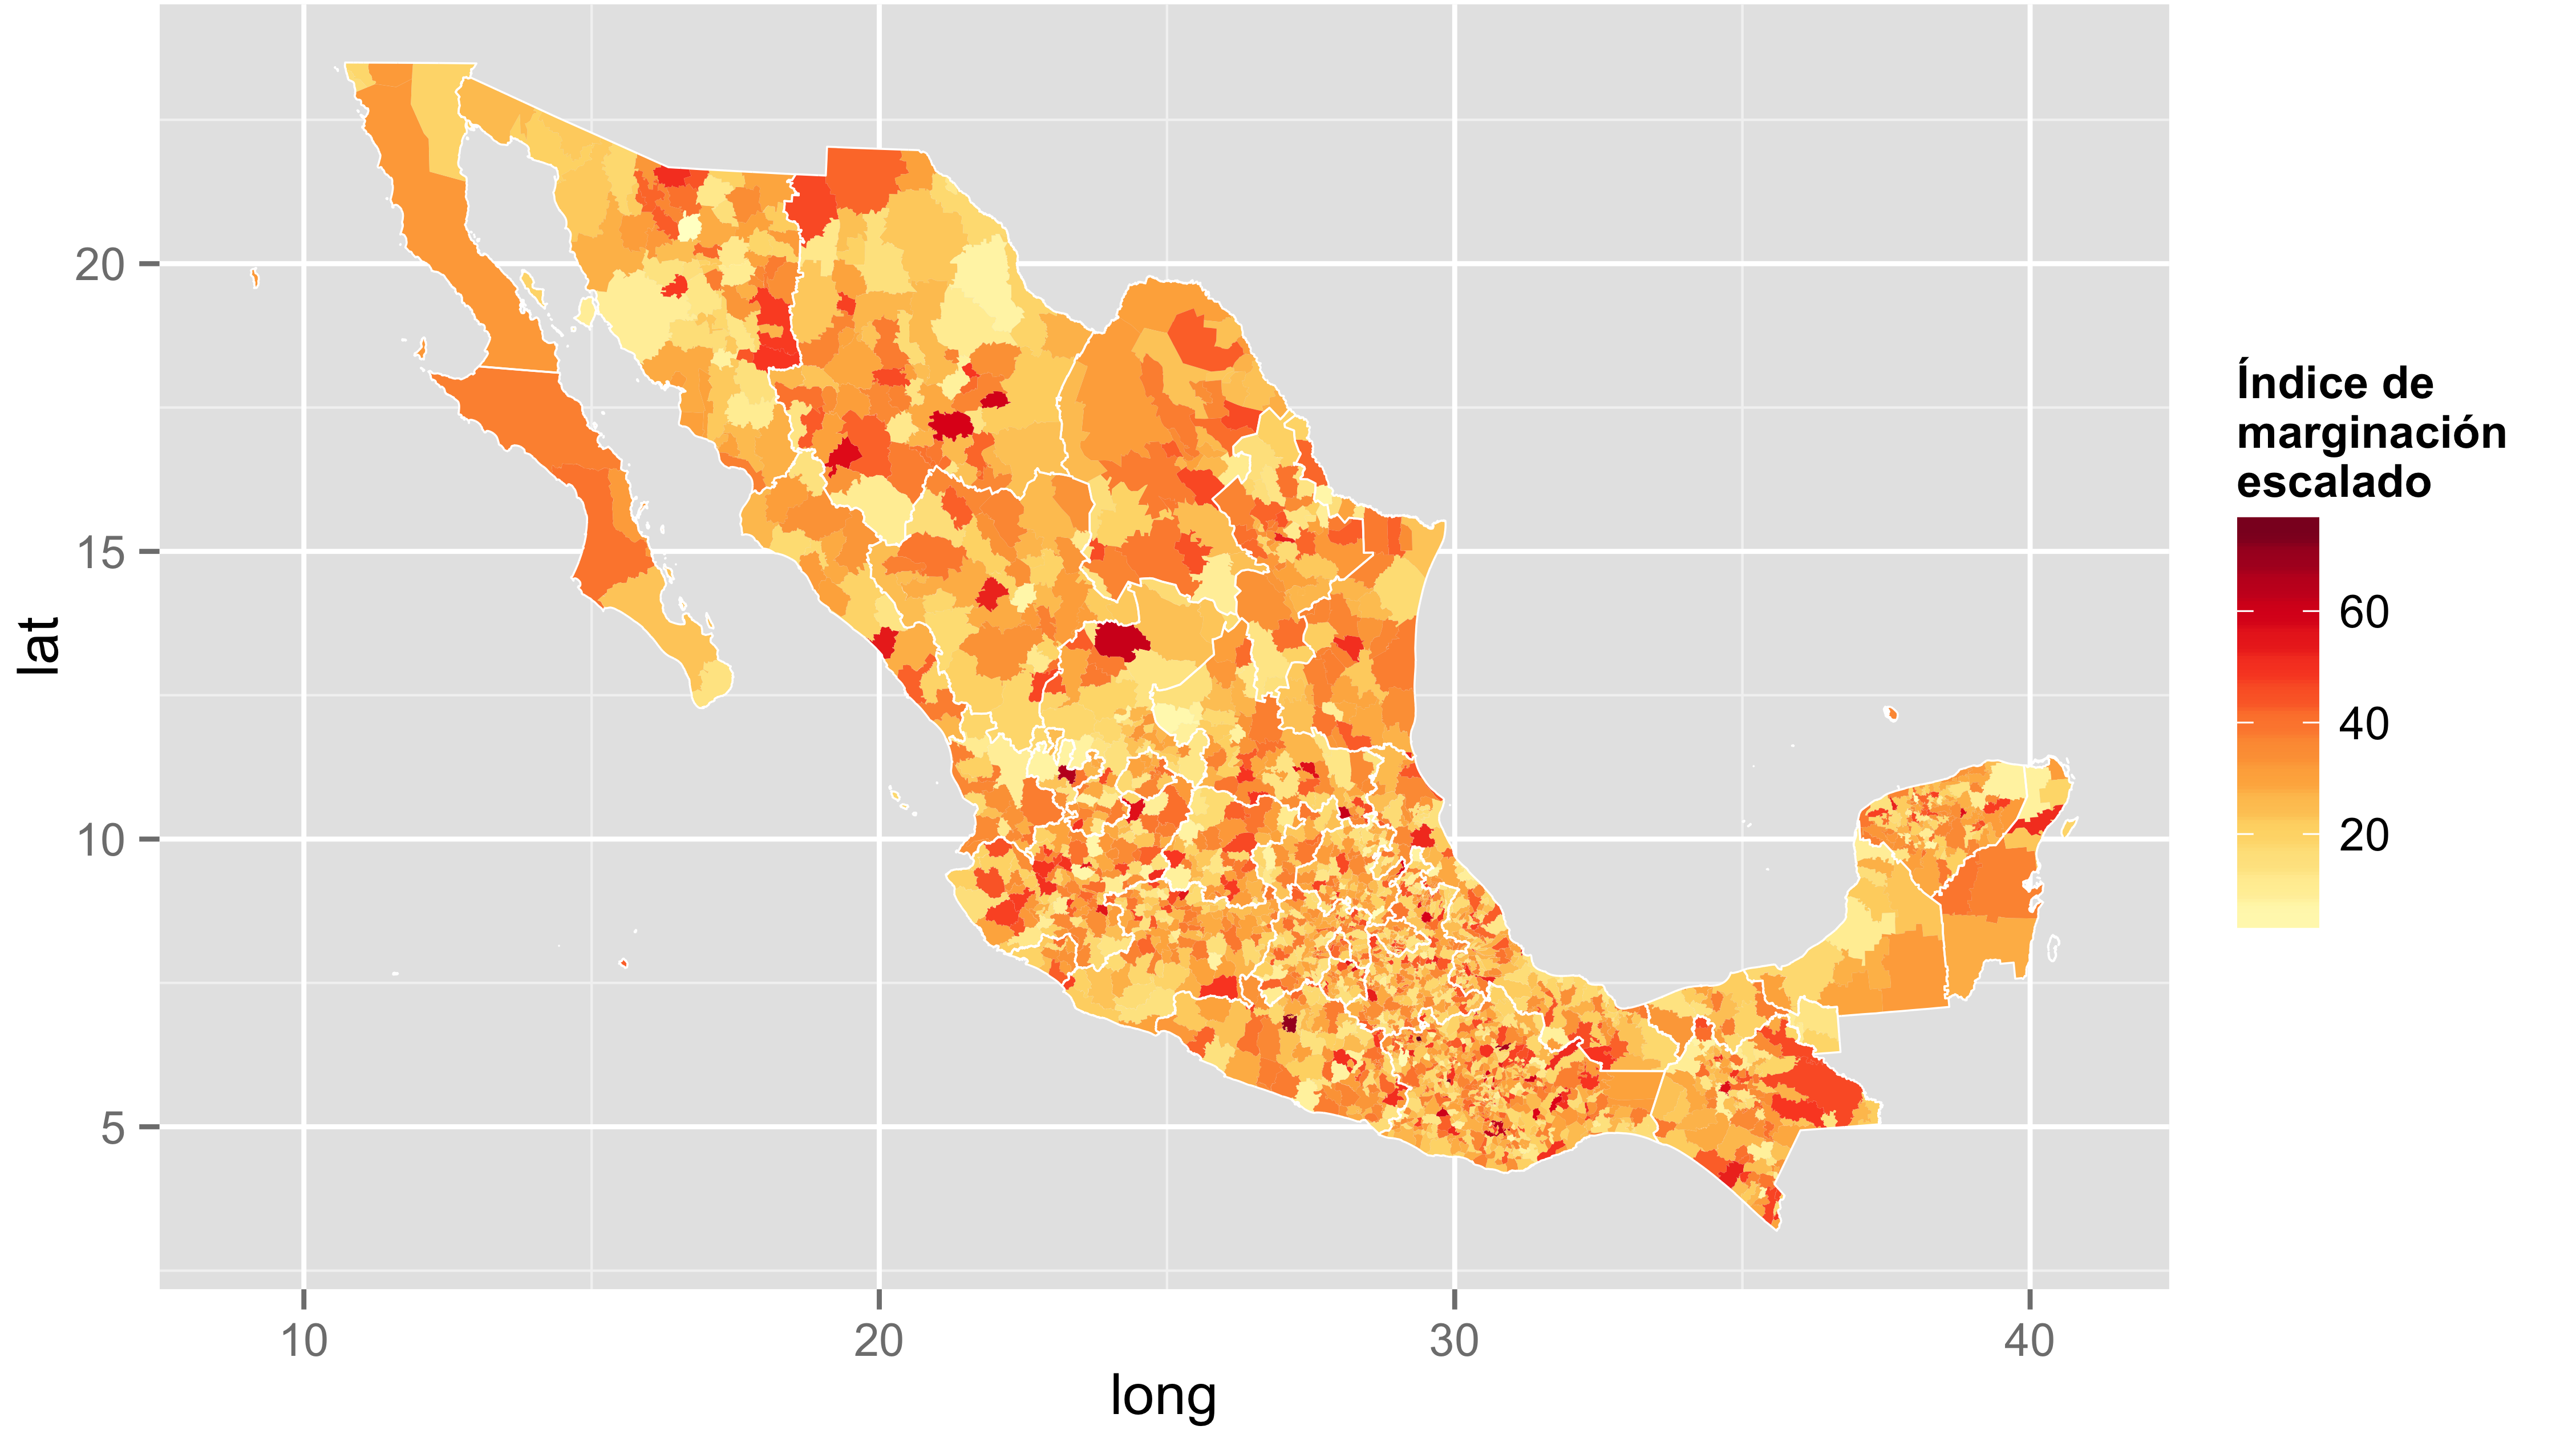
\includegraphics[width=\textwidth]{./maps/rmapmarg.png} \\
      \caption{ Permutación aleatoria del índice de marginación por municipio.}
      \label{rmap_marg_ej}  
    \end{figure}

    \item Calculamos el estadístico de interés, digamos $\mathcal{I}$, con las etiquetas permutadas. Si la variable $Y$ es continua hay $n!$ permutaciones posibles; si es discreta, $\dbinom{n}{n_1 n_2 \dots n_k}$.
    \item Repetimos 1. y 2. $n_{sim}$ veces, obteniendo una muestra de tamaño $n_{sim}$ de $\mathcal{I}$. 
    \item Comparamos el valor observado del estadístico con la muestra obtenida. Si la hipótesis alternativa. Si la $\mathcal{I}$ observada cae en un área mayor a $(1-\alpha)\%$ o menor a $\alpha\%$, entonces $\mathcal{I}$ es significativamente (positivo o negativo) a un nivel de significancia $\alpha$.
    \end{enumerate}


\subsection{Diagrama de dispersión de Moran} 
Un enfoque para visualizar asociación espacial se basa en el concepto del diagrama de dispersión de Moran propuesto por \citet{anselin93} que compara la variable de interés $y_i$  contra su retraso espacial (promedio ponderado de $Y$ en las regiones vecinas de $i$), para $i=1,2,\dots,n$. 

Si restamos $\bar{y}$ a ambos valores, la nube queda partida por los ejes en cuatro cuadrantes. Puntos en los cuadrantes Alto-Alto y Bajo-Bajo indican autocorrelación espacial positiva; mientras que puntos los cuadrantes Alto-Bajo y Bajo-Alto, autocorrelación espacial negativa.

Si colocamos el retraso espacial en el eje vertical y el valor en cada región en el eje de horizontal, el índice $\mathcal{I}$ corresponde a la pendiente de la línea de regresión ajustada.



%\begin{figure}
%\centering
%\vspace{2.0in}
%\caption[A Shorter Caption for the List of Figures]
%   {This is the Caption for the First Figure in Chapter 2.  It is a
%    long, long caption; we do not want to put the whole thing in the
%    List of Figures. A Shorter Caption can go in the square brackets.}
%% If you like additional lines in the caption indented, see the root template
%% file rpithes.tex for an example of using the caption package to do this.
%\end{figure}
% 
%This is a sentence to take up space and look like text.
%This is a sentence to take up space and look like text.
%This is a sentence to take up space and look like text.
%This is shown in table~\ref{mytable}.  % see \label below
% 
%\begin{table}
%\caption{This is the Caption for Table 2}
%\label{mytable}        % \label command must always comes AFTER the caption
%\begin{center}
%\begin{tabular}{lll}
%Here's       & another     & example  \\
%of           & a           & table    \\
%floated      & with        & the      \\
%\verb+table+ & environment & command.
%\end{tabular}
%\end{center}
%\end{table}
% 
%This is a sentence to take up space and look like text.
%This is a sentence to take up space and look like text.
% 
%\section{This is a Section Heading}
% 
%This is a sentence to take up space and look like text.
%This is a sentence to take up space \cite{yetanotherbook}.
%This is a sentence to take up space and look like text.
%This is a sentence to take up space and look like text.
% 
%\subsection{This is a Subsection Heading} 
% 
%This is a sentence to take up space and look like text.
%This is a sentence to take up space and look like text.
%This is a sentence to take up space and look like text.
%Text before a footnote.\footnote{Here's the text 
%of the footnote.}
%Text after the footnote.
% 
%This is a sentence to take up space and look like text.
%This is a sentence to take up space and look like text.
%Text before another footnote.\footnote{Here's the 
%text of the footnote.}
%Text after the footnote.
%This is a sentence to take up space and look like text.
%
%%%% Local Variables: 
%%%% mode: latex
%%%% TeX-master: t
%%%% End: 
